\chapter{一元多项式和高次方程}

\section{一元$n$次多项式}

\subsection{一元$n$次多项式}

形如$a_nx^n+a_{n-1}x^{n-1}+a_{n-2}x^{n-2}+\cdots+a_1x+a_0$.(其中$a_n\ne 0$)的代数式,叫做以$x$为元的一元$n$次多项式. $n$为确定的自然数.

我们把系数$a_i\; (i=0,1,\ldots,n)$都是复数的一元$n$次多项式叫做\textbf{复系数一元$n$次多项式}. 类似地,把系数都是实数(或有理数、整数等)的一元$n$次多项式叫做\textbf{实系数(或有理系数、整系数等)一元$n$次多项式},它们都是复系数一元$n$次多项式的特殊情形. 在本章中提到的多项式,如果不特别说明,都是指复系数多项式.

单独的一个非零数$a_0$,可以看作\textbf{零次多项式}(事实上,当$x\ne 0$时,$a_0=a_0x^0$). 系数都是零的多项式叫做\textbf{零多项式},零多项式没有确定的项数与次数.

\subsection{两个多项式相等的充要条件}

两个多项式相等的充要条件是它们的对应项系数相等(或两个多项式的差为零多项式). 这是待定系数法的理论依据.

\subsection{多项式的值}
一元$n$次多项式$f(x)=a_nx^n+a_{n-1}x^{n-1}+a_{n-2}x^{n-2}+\cdots+a_1x+a_0\; (a_n\ne 0)$,当$x$取复数集$\mathbb{C}$上的某一个值$a+bi\; (a,b\in\R)$时,都有其确定的值,记作$f(a+bi)$. $f(a+bi)$称为当$x=a+bi$时多项式$f(x)$的值. 很明显,无论$x$在$C$上取什么值,零多项式的值恒为零.故零多项式可记作数0.

\subsection{多项式的根}
如果$x=a$时,$f(a)=0$. 则称$a$为多项式$f(x)$的根(或零点).

\section{综合除法}
\subsection{带余除法}
一元多项式相加(包括相减)、相乘的结果仍是一元多项式,并且加、乘运算满足交换律、结合律以及乘法对加法的分配律.

一个一元多项式除以另一个一元多项式,并不是总能整除,当被除式$f(x)$除以除式$g(x)$(不是零多项式),得商式
$q(x)$及余式$r(x)$时,就有下列等式:
\[f(x)=g(x)q(x)+r(x)\]
其中$r(x)$的次数小于$g(x)$的次数,或者$r(x)$是零多项式. 当$r(x)$是零多项式时,就是$f(x)$能被$g(x)$整除.

\subsection{综合除法}
一个一元多项式除以一个一元一次式,有一种简便的计算方法——综合除法.

先用一般的除法来计算$a_3x^3+a_2x^2+a_1x+a_0$除以$x-b$:

\begin{center}
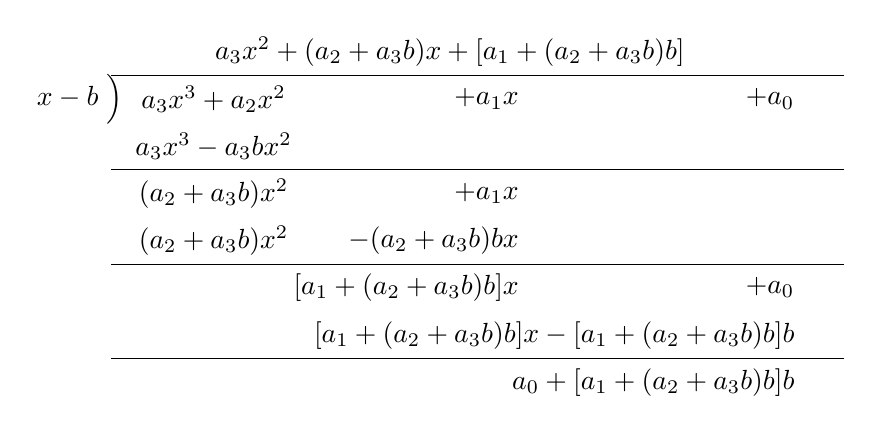
\begin{tikzpicture}[yscale=.6]

\node at (3,6){$a_3x^2+(a_2+a_3b)x+[a_1+(a_2+a_3b)b]$};
\foreach \x/\y in {5/a_3x^3+a_2x^2, 4/a_3x^3-a_3bx^2, 3/(a_2+a_3b)x^2, 2/(a_2+a_3b)x^2}
{
    \node at (0,\x){$\y$};
}
\foreach \x/\y in {5/+a_1x, 3/+a_1x, 2/-(a_2+a_3b)bx, 1/[a_1+(a_2+a_3b)b]x}
{
    \node at (4,\x)[left]{$\y$};
}
\foreach \x/\y in {5/+a_0, 1/+a_0, 0/[a_1+(a_2+a_3b)b]x-[a_1+(a_2+a_3b)b]b, -1/a_0+[a_1+(a_2+a_3b)b]b}
{
    \node at (7.5,\x)[left]{$\y$};
}

\foreach \x in {5.5,3.5,1.5,-.5}
{
    \draw(-1.3,\x)--(8,\x);
}
\node at (-1.7,5){$x-b\; \Big)$};
\end{tikzpicture}
\end{center}

这里所得的商式是$a_3x^2+(a_2+a_3b)x+[a_1+(a_2+a_3b)b]$;余式是$a_0+[a_1+(a_2+a_3b)b]b$,
它不含$x$,所以它是一个常数,下面把它叫做余数.

商式中各项的系数及余数分别是
\[a_3,\quad a_2+a_3b,\quad a_1+(a_2+a_3b)b\quad 
a_0+[a_1+(a_2+a_3b)b]b\]
其中第一个数就是被除式中第一项的系数,把这个数乘以$b$再加上被除式中下一项的系数就得第二个数,依此类推,最后得到余数.

因此,上面的除法可以用下面的简便算式来进行:
\begin{center}
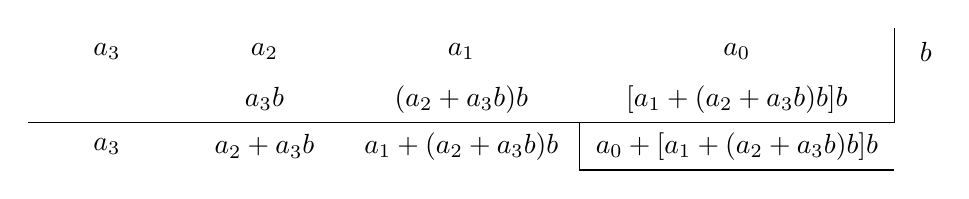
\begin{tikzpicture}[yscale=.6, xscale=2]
\foreach \x/\y in {1/a_3,2/a_2,3.25/a_1,5/a_0,6.2/b}
{
    \node at (\x,3){$\y$};
}
\foreach \x/\y in {2/a_3b,3.25/(a_2+a_3b)b,5/[a_1+(a_2+a_3b)b]b}
{
    \node at (\x,2){$\y$};
}
\foreach \x/\y in {1/a_3,2/a_2+a_3b,3.25/a_1+(a_2+a_3b)b,5/a_0+[a_1+(a_2+a_3b)b]b}
{
    \node at (\x,1){$\y$};
}

\draw(.5,1.5)--(6,1.5)--(6,3.5);
\draw(4,1.5)--(4,.5)--(6,.5);
\end{tikzpicture}
\end{center}

这里,第一行是被除式按降幂排列时各项的系数,如果有缺项,必须用零补足. 移下第一个系数,乘以$b$,加上第二个系数,依次进行,算得的第三行就是商式各项的系数及余数. 用这种算式进行的除法叫做\textbf{综合除法}.

被除式的次数不是三次时,综合除法同样适用.

\begin{example}
用综合除法计算:
\begin{enumerate}[(1)]
    \item $(\polynomial[reciprocal]{1,8,-2,-14})\div (x+1)$
    \item $(\polynomial[reciprocal]{2,5,-24,0,15})\div(x-2)$
\end{enumerate}
\end{example}

\begin{solution}
\begin{enumerate}[(1)]
    \item $x+1$就是$x-(-1)$
\begin{center}
    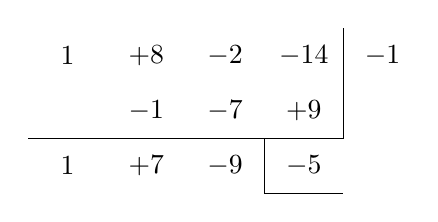
\begin{tikzpicture}[yscale=.7]
\foreach \x/\y in {1/1,2/+8,3/-2,4/-14,5/-1}
{
    \node at (\x,3){$\y$};
}
\foreach \x/\y in {2/-1,3/-7,4/+9}
{
    \node at (\x,2){$\y$};
}
\foreach \x/\y in {1/1,2/+7,3/-9,4/-5}
{
    \node at (\x,1){$\y$};
}
\draw(.5,1.5)--(4.5,1.5)--(4.5,3.5);
\draw(3.5,1.5)--(3.5,.5)--(4.5,.5);

    \end{tikzpicture}
\end{center}
$\therefore\quad $商式是$\polynomial[reciprocal]{1,7,-9}$,余数是$-5$.
    \item 被除式缺一次项,用0补足,得
 \begin{center}
    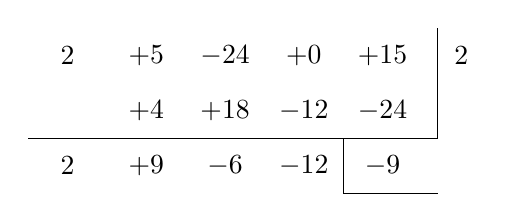
\begin{tikzpicture}[yscale=.7]
\foreach \x/\y in {1/2,2/+5,3/-24,4/+0,5/+15, 6/2}
{
    \node at (\x,3){$\y$};
}
\foreach \x/\y in {2/+4,3/+18,4/-12, 5/-24}
{
    \node at (\x,2){$\y$};
}
\foreach \x/\y in {1/2,2/+9,3/-6,4/-12, 5/-9}
{
    \node at (\x,1){$\y$};
}
\draw(.5,1.5)--(5.7,1.5)--(5.7,3.5);
\draw(4.5,1.5)--(4.5,.5)--(5.7,.5);

    \end{tikzpicture}
\end{center}
$\therefore\quad $商式是$\polynomial[reciprocal]{2,9,-6,-12}$,余数是$-9$. 

\end{enumerate}
\end{solution}

\begin{example}
用综合除法计算下列各式,并把结果写成“$f(x)=g(x)q(x)+r(x)$”的形式:
\begin{enumerate}[(1)]
    \item $(\polynomial[reciprocal]{4,0,-7,7,5})\div \left(x-\frac{3}{2}\right)$
    \item $(\polynomial[reciprocal]{6,-5,-3,-1,4})\div (2x+1)$
\end{enumerate}
\end{example}

\begin{solution}
\begin{enumerate}[(1)]
    \item 
\begin{center}
    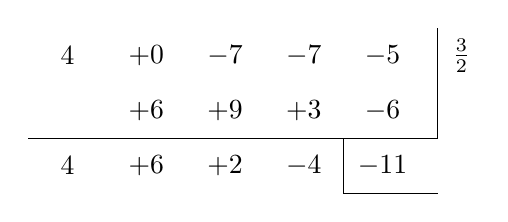
\begin{tikzpicture}[yscale=.7]
\foreach \x/\y in {1/4,2/+0,3/-7,4/-7,5/-5, 6/\frac{3}{2}}
{
    \node at (\x,3){$\y$};
}
\foreach \x/\y in {2/+6,3/+9,4/+3, 5/-6}
{
    \node at (\x,2){$\y$};
}
\foreach \x/\y in {1/4,2/+6,3/+2,4/-4, 5/-11}
{
    \node at (\x,1){$\y$};
}
\draw(.5,1.5)--(5.7,1.5)--(5.7,3.5);
\draw(4.5,1.5)--(4.5,.5)--(5.7,.5);

    \end{tikzpicture}
\end{center}
$\therefore\quad \polynomial[reciprocal]{4,0,-7,7,5}=\left(x-\frac{3}{2}\right)(\polynomial[reciprocal]{4,6,2,-4})-11$.

\item $2x+1$就是$2\left(x+\frac{1}{2}\right)$,先将
$\polynomial[reciprocal]{6,-5,-3,-1,4}$除以$x+\frac{1}{2}$.
\begin{center}
    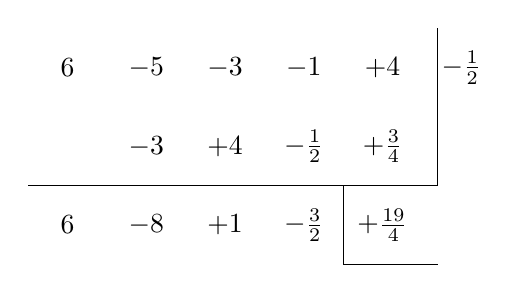
\begin{tikzpicture}[yscale=1]
\foreach \x/\y in {1/6,2/-5,3/-3,4/-1,5/+4, 6/-\frac{1}{2}}
{
    \node at (\x,3){$\y$};
}
\foreach \x/\y in {2/-3,3/+4,4/-\frac{1}{2}, 5/+\frac{3}{4}}
{
    \node at (\x,2){$\y$};
}
\foreach \x/\y in {1/6,2/-8,3/+1,4/-\frac{3}{2}, 5/+\frac{19}{4}}
{
    \node at (\x,1){$\y$};
}
\draw(.5,1.5)--(5.7,1.5)--(5.7,3.5);
\draw(4.5,1.5)--(4.5,.5)--(5.7,.5);

    \end{tikzpicture}
\end{center}
\[\begin{split}
    \therefore\quad \polynomial[reciprocal]{6,-5,-3,-1,4}&=\left(x+\frac{1}{2}\right)\left(\polynomial[reciprocal]{6,-8,1,-\frac{3}{2}}\right)+\frac{19}{4}\\
    &=2\cdot \left(x+\frac{1}{2}\right)\cdot \frac{1}{2}\left(\polynomial[reciprocal]{6,-8,1,-\frac{3}{2}}\right)+\frac{19}{4}\\
    &=(2x+1)\left(\polynomial[reciprocal]{3,-4,\frac{1}{2},-\frac{3}{4}}\right)+\frac{19}{4}\\
\end{split}\]

\end{enumerate}
\end{solution}

由例9.2的第(2)小题可知,$f(x)$除以一般的一元一次式$px\pm q$,也可以使用综合除法:先将$f(x)$除以$x\pm\frac{q}{p}$,所得的商式除以$p$就是所求的商式,所得的余数就是所求的余数.

\begin{ex}
    用综合除法计算(第1—3题):
\begin{enumerate}
    \item $(x^{3}+6x^{2}-11x-14)\div(x-3).$
    \item $\left(x^{5}-4x^{3}-8\right)\div\left(x-2\right).$
    \item $(3x^{4}+7x^{3}-15x-20)\div(x+2).$
\end{enumerate}

用综合除法计算下列各式,并且把所得的结果写成
“$f(x)=g(x)q(x)+r(x)$”的形式(第4—6题):
\begin{enumerate}\setcounter{enumi}{3}
    \item $( x^{6}+ 1) \div ( x+ 1) .$
    \item $(27x^{3}-10)\div(3x-2).$
    \item $\left(20x^{5}+9x^{4}-8x^{3}+12x^{2}-35x-12\right)\div\left(5x+6\right).$
\end{enumerate}
\end{ex}





\section{余数定理}

设有多项式 $f(x)=x^3-7x^2+12x+27$, 那么 $f(5)=5^3 -7\times5^{2}+12\times5+27=125-175+60+27=37;$另一方面,如果把这个多项式除以 $x-5$, 求余数,那么用综合除法可得
\begin{center}
    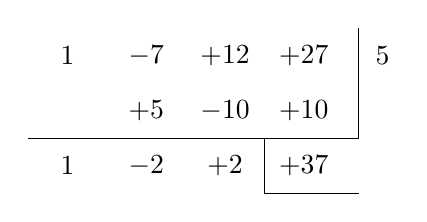
\begin{tikzpicture}[yscale=.7]
\foreach \x/\y in {1/1,2/-7,3/+12,4/+27,5/5}
{
    \node at (\x,3){$\y$};
}
\foreach \x/\y in {2/+5,3/-10,4/+10}
{
    \node at (\x,2){$\y$};
}
\foreach \x/\y in {1/1,2/-2,3/+2,4/+37}
{
    \node at (\x,1){$\y$};
}
\draw(.5,1.5)--(4.7,1.5)--(4.7,3.5);
\draw(3.5,1.5)--(3.5,.5)--(4.7,.5);

    \end{tikzpicture}
\end{center}
我们发现,所得的余数正好也是 37. 这就是说,多项式$f(x)=
x^3-7x^2+12x+27$ 除以 $x-5$ 所得的余数正好等于$f(5)$.

对一般的多项式,有下面的重要定理:

\begin{thm}{余数定理}
    多项式$f(x)$除以$x-b$所得的余数等于$f(b)$.
\end{thm}

\begin{proof}
    设多项式$f(x)$除以$x-b$所得的商式为$q(x)$,余数为$r$,则有
\[f(x)=(x-b)\cdot q(x)+r\]
用$x=b$代入等式的两边,得
\[f(b)=(b-b)\cdot q(b)+r\]
由此即得余数$r=f(b)$.
\end{proof}

根据余数定理\footnote{此定理又叫做余式定理、剩余定理或裴蜀定理. 裴蜀(\'{E}tienne B\'{e}zout, 1730—1783),法国数学家.},既然多项式$f(x)$除以$x-b$所得的余数$r$等于$f(x)$在$x=b$时的值$f(b)$,那么$r$就可以由$f(b)$来求得,反过来,$f(b)$也可以由$r$来求得.

\begin{example}
    设$f(x)=x^8+3$,求$f(x)$除以$-1$所得的余数.
\end{example}

\begin{solution}
    根据余数定理,所求的余数等于$f(-1)=(-1)^8+3=4$.
\end{solution}

\begin{example}
    设$f(x)=x^5-12x^3+15x-8$,求$f(6)$.
\end{example}

\begin{solution}
    用综合除法求$f(x)$除以$x-6$所得的余数:
\begin{center}
    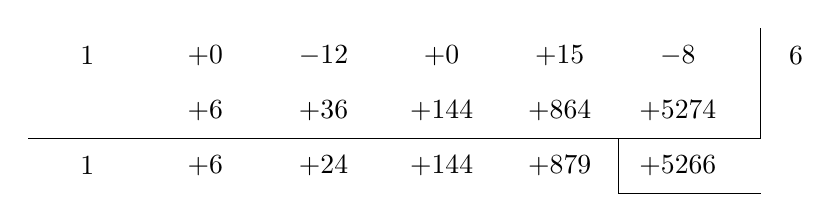
\begin{tikzpicture}[xscale=1.5, yscale=.7]
\foreach \x/\y in {1/1,2/+0,3/-12,4/+0,5/+15, 6/-8, 7/6}
{
    \node at (\x,3){$\y$};
}
\foreach \x/\y in {2/+6,3/+36,4/+144, 5/+864, 6/+5274}
{
    \node at (\x,2){$\y$};
}
\foreach \x/\y in {1/1,2/+6,3/+24,4/+144, 5/+879, 6/+5266}
{
    \node at (\x,1){$\y$};
}
\draw(.5,1.5)--(6.7,1.5)--(6.7,3.5);
\draw(5.5,1.5)--(5.5,.5)--(6.7,.5);
    \end{tikzpicture}
\end{center}

根据余数定理,余数5266等于$f(6)$,所以
$f(6)=5266$. 
\end{solution}

\begin{ex}
\begin{enumerate}
 \item 设$f(x)=5x^4-x^2+6$, 求$f(x)$除以$x-1$所得的余数.
\item 设$f(x)=x^4-3x^{3}+6x^{2}-10x+9$, 求$f(4)$.
\item 已知$f( x) = 16x^4- 14x^{3}- 15x^{2}- 24x+ 38$, 求$f\left ( \frac 32\right )$.
\item 设$f(x)=x^6+a^6$, 求$f(x)$除以$x-ai$所得的余数.
\end{enumerate}
\end{ex}

\section{因式定理}

从余数定理可以推出一个重要的定理——因式定理。

\begin{thm}
 {因式定理} 多项式$f(x)$有一个因式$x-b$的充要条件是
$f(b)=0$.   
\end{thm}

\begin{proof}
\begin{enumerate}[(1)]
\item 充分性. 设 $f(b)=0$, 则根据余数定理, $f(x)$除以$x-b$所得的余数也等于 0. 因此$f(x)$有一个因式$x-b$.
\item 必要性. 设 $f(x)$有一个因式 $x-b$, 则 $f(x)$除以 $x-b$
所得的余数等于 0. 根据余数定理,有$f(b)=0$.
\end{enumerate}
\end{proof}

\begin{example}
    求证$n$为任何正整数时,$x^n-a^n$都有因式$x-a$.
\end{example}

\begin{proof}
    设$f(x)=x^n-a^n$, 那么$f(a)=a^n-a^n=0$. 根据因
式定理, $x^*-a^*$有因式$x-a$.
\end{proof}

\begin{example}
    $m$为何值时,多项式$f(x)=x^5-3x^4+8x^3+11x+$
$m$能被$x-1$整除?
\end{example}

\begin{solution}
    $f(x)$能被 $x- 1$ 整除, 就是 $f(x)$有因式 $x-1$. 根据因式定理,充要条件是$f(1)=0$, 即$1-3+8+11+m=0$. 由此可得$m=-17$.
\end{solution}

\begin{ex}
\begin{enumerate}
\item 不用除法,求证多项式$x^4-5x^3-7x^2+15x-4$有因式
$x-1$.
\item 求证$n$为正偶数时, $x^n-a^n$有因式$x+a$; $n$为正奇数时, $x^n+a^{n}$有因式$x+a$.
\item 求证 $x^{in}-1\; (n\in \N)$有因式 $x-i$, 又有因式 $x+i$. 
\item 已知$f(x)=x^3-8x+\ell$有因式$x+2$, 确定$\ell$的值.
\end{enumerate}    
\end{ex}

\section{利用综合除法、因式定理来分解因式}

设有多项式 $x^6+x^4-x^2-1$, 我们把它在复数集$\mathbb{C}$ 中分
解因式,得
\[\begin{split}
    x^{6}+x^{4}-x^{2}-1&=x^{4}(x^{2}+1)-(x^{2}+1)\\
    &=(x^{4}-1)(x^{2}+1)\\
    &=(x^{2}-1)(x^{2}+1)(x^{2}+1)\\
    &=(x+1)(x-1)(x+i)^{2}(x-i)^{2}.
\end{split}\]

这个一元六次式有六个一次因式,其中有两个相同因式
$x+i$, 两个相同因式$x-i$.

关于复系数一元$n$次多项式的因式分解,有下面的定理: 

\begin{thm}
{定理1} 任何一个复系数一元 $n$ 次多项式 $f(x)$有且仅有
$n$ 个 一 次 因 式 $x- x_i\; ( i= 1, 2, \cdots , n)$, 把其中相同的因式的积用幂表示后, $f(x)$就具有唯一确定\footnote{这里所说的“唯一确定”,不考虑各一次因式的书写顺序,也不考虑常数因子. 例如,我们把$4x^2-16=(2x+4)(2x-4)$与$4x^2-16=4(x-2)(x+2)$等等看成同一种分解形式.}的因式分解的形式:
\begin{equation}
    f( x) = a_{x}( x- x_{1}) ^{k_{1}}( x- x_{2}) ^{k_{2}}\cdots ( x- x_{m}) ^{k_{m}} \tag{*}
\end{equation}   
其中 $k_1,k_2,\ldots,k_m\in \N$, 且 $k_1+k_2+\cdots+k_m=n$, 复数 $x_1,x_2,\ldots,x_{m}$两两不等.
\end{thm}

这个定理的证明超出中学数学范围,本书从略。

我们把分解结果(*)中的$x-x_i\; (i=1,2,\ldots,m)$叫做\textbf{多项式$f(x)$的$k_i$重一次因式}. 例如:多项式$x^2-6x+9$有 2 重一次因式 $x-3$; 多项式$(x-4)(x+2)^2(x-5)^3$ 有 1 重一次因式$x- 4$, 2重一次因式$x+ 2$, 3重一次因式$x-5$.

由定理 1 可以得到:

\begin{thm}
{推论} 如果 $x-a,x-b\; (a\neq0)$都是复系数一元$n$次多项式 $f(x)$的因式,那么它们的积$(x-a)(x-b)$也是 $f(x)$的因式.    
\end{thm}

\begin{proof}
因为 $f(x)$的分解结果(*)是唯一确定的,所以 $a$ 一定等于某个$x_i,b$一定等于某个$x_j\; (i=1,2,\ldots,m,\; j=1,2,\ldots,m, \text{ 且 } i\neq j)$, 即$(x-a)(x-b)=(x-x_{i})(x-x_j)$, 由此可见, $(x-x_i)(x-x_j)$是 $f(x)$的因式.    
\end{proof}

对于一个任意的复系数一元$n$次多项式$f(x)$, 要求出它的一次因式,没有一般的方法. 但是,如果 $f(x)$是整系数多项式,那么进一步运用下列定理,就能使我们较快地求得它的形如$x-\frac qp$(其中$p,q$是互质的整数)的因式,或者确定它没有这种形式的因式.

\begin{thm}
    {定理2} 如果整系数多项式$f(x)=a_nx^n+a_{n-1}x^{n-1}+\cdots+a_{1}x+a_{0}$有因式 $x-\frac qp$(其中 $p,q$ 是互质的整数),那么 $p$一定是首项系数$a$的约数,$q$一定是末项系数$a_0$的约数.
\end{thm}

例如,$15x^2-17x+4$ 有因式 $3x-1$, $5x-4$, 即$3\left(x-\frac{1}{3}\right)$, $5\left(x-\frac{4}{5}\right)$,3与5都是首项系数15的约数,1与4都是末项
系数4的约数. 又如,如果$2x^4-x^3-13x^2-x-15$有$x-\frac qp$形式的因式(其中$p,q$是互质的整数,下同),那么$p$只可能是$1,2$,$q$只可能是$\pm1,\pm3,\pm5,\pm15$.

要注意定理中“$p$ 是$a_n$的约数,$q$ 是$a_0$的约数”只是“整系数多项式$a_nx^n+a_{n-1}x^{n-1}+\cdots+a_1x+a_0$有因式$x-\frac qp$”的必要条件,而不是充分条件(为什么).

下面证明定理 2.

\begin{proof}
因为 $f(x)$有因式 $x-\frac qp$, 所以 $f\left(\frac qp\right)=0$, 即
$$a_{n}\Big(\frac{q}{p}\Big)^{n}+a_{n-1}\Big(\frac{q}{p}\Big)^{n-1}+\cdots+a_{1}\Big(\frac{q}{p}\Big)+a_{0}=0$$
把第二项起的各项移到右边,并将两边都乘以 $p^{n-1}$, 得
$$\frac{a_nq^n}p=-(a_{n-1}q^{n-1}+\cdots+a_1qp^{n-2}+a_0p^{n-1})$$

等式的右边是一个整数,所以$\frac{a_nq^n}p$也是一个整数,即$p$能整除$a_nq^n$. 但因$p,q$互质,所以$p$的任何一个质因数都不是$q$ 的约数,从而也不是$q^{n}$的约数\footnote{例如:$p=2\x 5=10$, $q=3\x 7=21$,$p$的任何一个质因数(2或5)都不是$q$的约数,从而也不是$q^n=3^n\x 7^n$的约数.}。由此可知,
$p$一定是$a_n$的约数。

同理,把上面的等式写成
$$\frac{a_{0}p^{n}}{q}=-\left(a_{n}q^{n-1}+a_{n-1}q^{n-2}p+\cdots+a_{1}p^{n-1}\right)$$
可以证明$q$一定是$a_0$的约数.
\end{proof}

\begin{thm}
    {推论} 如果首项系数为1的整系数多项式$f(x)=x^{n}+ a_{n-1}x^{n-1}+\cdots+a_1x+a_0$有因式 $x-q$, 其中 $q\in\mathbb{Z}$, 那么 $q$一定是常数项$a_0$的约数。
\end{thm}

利用定理 2 及其推论,我们可以较快地确定一个整系数
一元一次式是不是某整系数一元$n$次多项式的因式.

\begin{example}
    把$f(x)=x^3+x^2-10x-6$ 分解因式\footnote{如果没有特别说明,本章中所说的因式分解,都是指在复数集$\mathbb{C}$中的因
    式分解.}
\end{example}

\begin{analyze}
    先考虑 $x-q\; (q\in \Z)$形式的因式,因为 $f(x)$是首项系数为 1 的整系数多项式,根据定理 2 的推论,可能出现的$x-q$这样的因式有 $x\pm1$, $x\pm2$, $x\pm3$, $x\pm6$.

判断$x-1$, $x+1$是不是$f(x)$的因式时,只要根据因式定理,计算 $f(1)$, $f(-1)$是不是等于零就可以了. 因为 $f(1)=-14\neq0$, $f(-1)=4\neq0$, 所以 $x-1$, $x+1$ 都不是 $f(x)$的因式.

判断$x-2,x+2,\ldots$是不是$f(x)$的因式时,可以计算
$f(2),f(-2),\ldots$是不是等于零. 用综合除法,由于
\begin{center}
\begin{tikzpicture}[yscale=.7]
\begin{scope}
    \foreach \x/\y in {1/1,2/+1,3/-10,4/-6,5/2}
{
    \node at (\x,3){$\y$};
}
\foreach \x/\y in {2/+2,3/+6}
{
    \node at (\x,2){$\y$};
}
\foreach \x/\y in {1/1,2/+3,3/-4}
{
    \node at (\x,1){$\y$};
}
\draw(.5,1.5)--(4.5,1.5)--(4.5,3.5);
\end{scope}
\begin{scope}[xshift=6cm]
\foreach \x/\y in {1/1,2/+1,3/-10,4/-6,5/-2}
{
    \node at (\x,3){$\y$};
}
\foreach \x/\y in {2/-2,3/+2}
{
    \node at (\x,2){$\y$};
}
\foreach \x/\y in {1/1,2/-1,3/-8}
{
    \node at (\x,1){$\y$};
}
\draw(.5,1.5)--(4.5,1.5)--(4.5,3.5);
\end{scope}
\end{tikzpicture}
\end{center}
(上面左式中$-4\x2$不是$-6$的相反数,右式中$-8\x(-2)$不是$-6$的相反数,已经说明相应的余数都不是零,所以不必继续演算了.)可见$x-2$, $x+2$都不是$f(x)$的因式. 但
\begin{center}
    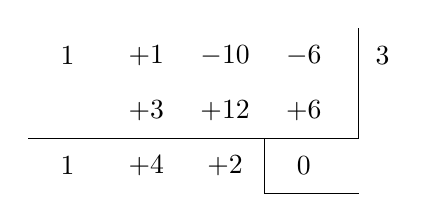
\begin{tikzpicture}[yscale=.7]
\foreach \x/\y in {1/1,2/+1,3/-10,4/-6,5/3}
{
    \node at (\x,3){$\y$};
}
\foreach \x/\y in {2/+3,3/+12, 4/+6}
{
    \node at (\x,2){$\y$};
}
\foreach \x/\y in {1/1,2/+4,3/+2, 4/0}
{
    \node at (\x,1){$\y$};
}
\draw(.5,1.5)--(4.7,1.5)--(4.7,3.5);
\draw(3.5,1.5)--(3.5,.5)--(4.7,.5);
\end{tikzpicture}
\end{center}
可知$x-3$是$f(x)$的因式. 所以
\[x^3+x^2-10x-6=(x-3)(x^2+4x+2)\]

因为方程$x^2+4x+2=0$的两个根是$-2\pm\sqrt{2}$,于是,
\[x^3+x^2-10x-6=(x-3)\left(x+2+\sqrt{2}\right)\left(x+2-\sqrt{2}\right)\]

解答时,只需写出结果是因式的试验过程,其他过程不必写出.
\end{analyze}

\begin{solution}
    \begin{center}
        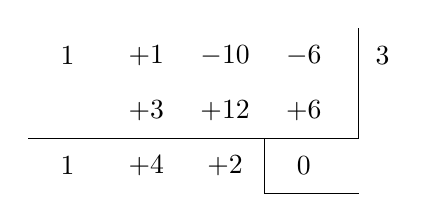
\begin{tikzpicture}[yscale=.7]
    \foreach \x/\y in {1/1,2/+1,3/-10,4/-6,5/3}
    {
        \node at (\x,3){$\y$};
    }
    \foreach \x/\y in {2/+3,3/+12, 4/+6}
    {
        \node at (\x,2){$\y$};
    }
    \foreach \x/\y in {1/1,2/+4,3/+2, 4/0}
    {
        \node at (\x,1){$\y$};
    }
    \draw(.5,1.5)--(4.7,1.5)--(4.7,3.5);
    \draw(3.5,1.5)--(3.5,.5)--(4.7,.5);
    \end{tikzpicture}
    \end{center}
\[\begin{split}
\therefore\quad x^3+x^2-10x-6&=(x-3)(x^2+4x+2)\\
&=(x-3)\left(x+2+\sqrt{2}\right)\left(x+2-\sqrt{2}\right)
\end{split}\]
\end{solution}

\begin{example}
把$f(x)=\polynomial[reciprocal]{2,-1,-13,-1,-15}$分解因式。
\end{example}

\begin{analyze}
$f(x)$首项系数不是1,根据定理2,可试验$x\pm1$, $x\pm3$, $x\pm5$, $x\pm15$, $x\pm\frac{1}{2}$, $x\pm\frac{3}{2}$, $x\pm\frac{5}{2}$, $x\pm\frac{15}{2}$. 

因为$f(1)\ne 0$, $f(-1)\ne 0$,所以$x+1$, $x-1$不是$f(x)$的因式. 但
\begin{center}
    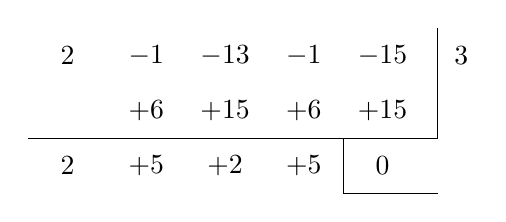
\begin{tikzpicture}[yscale=.7]
\foreach \x/\y in {1/2,2/-1,3/-13,4/-1,5/-15, 6/3}
{
    \node at (\x,3){$\y$};
}
\foreach \x/\y in {2/+6,3/+15, 4/+6, 5/+15}
{
    \node at (\x,2){$\y$};
}
\foreach \x/\y in {1/2,2/+5,3/+2, 4/+5, 5/0}
{
    \node at (\x,1){$\y$};
}
\draw(.5,1.5)--(5.7,1.5)--(5.7,3.5);
\draw(4.5,1.5)--(4.5,.5)--(5.7,.5);
\end{tikzpicture}
\end{center}

所以,$f(x)=(x-3)(2x^3+5x^2+2x+5)$.

继续分解$2x^3+5x^2+2x+5$. 这个多项式的首项系数是2,末项系数是5,所以只要试验$x\pm 1$, $x\pm 5$, $x\pm \frac{1}{2}$, $x\pm \frac{5}{2}$ 就可以了.但因$x\pm 1$不是原来多项式$f(x)$的因式,所以也不是这个多项式的因式. 由
\begin{center}
    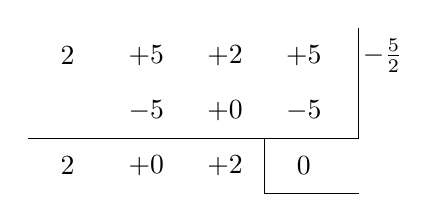
\begin{tikzpicture}[yscale=.7]
\foreach \x/\y in {1/2,2/+5,3/+2,4/+5,5/-\frac{5}{2}}
{
    \node at (\x,3){$\y$};
}
\foreach \x/\y in {2/-5,3/+0, 4/-5}
{
    \node at (\x,2){$\y$};
}
\foreach \x/\y in {1/2,2/+0,3/+2, 4/0}
{
    \node at (\x,1){$\y$};
}
\draw(.5,1.5)--(4.7,1.5)--(4.7,3.5);
\draw(3.5,1.5)--(3.5,.5)--(4.7,.5);
\end{tikzpicture}
\end{center}
得:
\[\begin{split}
\polynomial[reciprocal]{2,5,2,5}&=\left(x+\frac{5}{2}\right)(2x^2+2)\\
&=(2x+5)(x^2+1)
\end{split}\]
(实际上,利用分组分解法也容易得到这个结果.)

$x^2+1$在复数集$\mathbb{C}$中还能继续分解因式,所以
\[\begin{split}
    \polynomial[reciprocal]{2,-1,-13,-1,-15}&=(x-3)(2x+5)(x^2+1)\\
    &=(x-3)(2x+5)(x+i)(x-i)
\end{split}\]
\end{analyze}

\begin{solution}
\begin{center}
    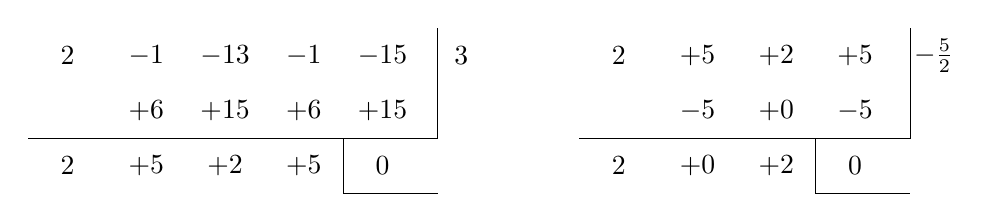
\begin{tikzpicture}[yscale=.7]
\begin{scope}
\foreach \x/\y in {1/2,2/-1,3/-13,4/-1,5/-15, 6/3}
{
    \node at (\x,3){$\y$};
}
\foreach \x/\y in {2/+6,3/+15, 4/+6, 5/+15}
{
    \node at (\x,2){$\y$};
}
\foreach \x/\y in {1/2,2/+5,3/+2, 4/+5, 5/0}
{
    \node at (\x,1){$\y$};
}
\draw(.5,1.5)--(5.7,1.5)--(5.7,3.5);
\draw(4.5,1.5)--(4.5,.5)--(5.7,.5);    
\end{scope}
\begin{scope}[xshift=7cm]
    \foreach \x/\y in {1/2,2/+5,3/+2,4/+5,5/-\frac{5}{2}}
{
    \node at (\x,3){$\y$};
}
\foreach \x/\y in {2/-5,3/+0, 4/-5}
{
    \node at (\x,2){$\y$};
}
\foreach \x/\y in {1/2,2/+0,3/+2, 4/0}
{
    \node at (\x,1){$\y$};
}
\draw(.5,1.5)--(4.7,1.5)--(4.7,3.5);
\draw(3.5,1.5)--(3.5,.5)--(4.7,.5);
\end{scope}
\end{tikzpicture}
\end{center}
\[\begin{split}
\therefore\quad \polynomial[reciprocal]{2,-1,-13,-1,-15}&=(x-3)(\polynomial[reciprocal]{2,5,2,5})\\
&=(x-3)(2x+5)(x^2+1)\\
&=(x-3)(2x+5)(x+i)(x-i)
\end{split}\]
\end{solution}

\begin{ex}
\begin{enumerate}
    \item 判断下列各命题的真假,并说明理由:
\begin{enumerate}[(1)]
\item 如果整数$p,q$互质,且$p$为整系数多项式
    $$f(x)=a_nx^n+a_{n-1}x^{n-1}+\cdots +a_1x+a_0$$
    的首项系数$a_n$的约数,$q$为末项系数$a_0$的约数,那么$x-\frac{q}{p}$一定是$f(x)$的因式;
\item 如果多项式$f(x)=g(x)q(x)$,其中$g(x)$, $q(x)$也是多项式,且$x-a$不是$f(x)$的因式,那么$x-a$也不是$q(x)$的因式.
\end{enumerate}
\item 把下列各式分解因式:
\begin{enumerate}[(1)]
    \item $\polynomial[reciprocal]{1,1,-10,8}$
    \item $\polynomial[reciprocal]{2,-9,1,12}$
    \item $\polynomial[reciprocal]{1,3,-3,-12,-4}$
    \item $\polynomial[reciprocal]{4,-13,10,-42,20}$
\end{enumerate}
\end{enumerate}
\end{ex}

\section*{习题一}
\begin{enumerate}
    \item 设$f(x)=\polynomial[reciprocal]{1,-i,2,-2i}$,求:
\begin{multicols}{3}
\begin{enumerate}[(1)]
    \item $f(0)$
    \item $f(2)$
    \item $f(i)$
    \item $f\left(\sqrt{2}i\right)$
    \item $f\left(-\sqrt{2}i\right)$
\end{enumerate}
\end{multicols}

\item 用综合除法求商式及余数:
\begin{enumerate}[(1)]
    \item $(\polynomial[reciprocal]{3,0,-50,0,14})\div (x-4)$
    \item $(\polynomial[reciprocal]{1,0,-15,-10,28})\div (x+2)$
    \item $(\polynomial[reciprocal]{3,-5,8,-1,-40})\div \left(x-\frac{2}{3}\right)$
    \item $(\polynomial[reciprocal]{1,6,9,0,-14,8})\div (x+4)$
    \item $(\polynomial[reciprocal]{5,-6,7,8})\div (5x+4)$
    \item $(\polynomial[reciprocal]{4,6,-8,5,0})\div (2x+5)$
    \item $(\polynomial[reciprocal, var=y]{1,-8,16,-25})\div (y-6)$
    \item $(\polynomial[reciprocal, var=a]{2,0,-1,9,-12})\div (a-2)$
    \item $(\polynomial[reciprocal, var=t]{8,14,-3,-35,18})\div (4t-3)$
    \item $(\polynomial[reciprocal, var=m]{25,0,36,-14,8,8})\div (5m+2)$
    \item $(x^3-8x^2y+8y^3)\div (x-2y)$ 
    
    (提示:把$x$看作多项式的元,$y$看作系数)
    \item $(10m^5-7m^4n-16m^3n^2+23mn^4-21n^5)\div (2m-3n)$
\end{enumerate}

\item \begin{enumerate}[(1)]
    \item 用综合除法求$f(x)=x^5-2x^4-5x^3+9x^2-14x+29$
    除以$x-3$所得的余数;
    \item 对于上题中的$f(x)$,用代入法求$f(3)$;
    \item 比较第(1),(2)小题所得的结果.
\end{enumerate}

\item \begin{enumerate}[(1)]
    \item 用综合除法求$f(x)=x^8-23x^4+19$除以$x+1$所得的余数;
\item 对于第(1)小题中的$f(x)$,用代入法求$f(-1)$;
\item 比较第(1),(2)小题所得的结果.
\end{enumerate}

\item \begin{enumerate}[(1)]
    \item 已知$f(x)=\polynomial[reciprocal]{1,2,-19,19,-25,-70}$,利用综合除法求$f(3)$;
    \item 已知$f(x)=\polynomial[reciprocal]{9,3,-32,10,27,-6}$,利用综合除法求$f\left(\frac{4}{3}\right)$;
\end{enumerate}

\item 不用除法,求下列各式除以$x-y$所得的余式以及除以$x+y$所得的余式:
\begin{multicols}{2}
\begin{enumerate}[(1)]
    \item $x^7+y^7$
    \item $x^7-y^7$
    \item $x^8+y^8$
    \item $x^8-y^8$
\end{enumerate}
\end{multicols}
\item 不用除法,求证:
\begin{enumerate}[(1)]
    \item $\polynomial[reciprocal]{5,0,4,-11,9,-3}$有因式$x-1$
    \item $\polynomial[reciprocal]{1,-8,-6,9,6}$有因式$x+1$
    \item $(x-1)^5-1$有因式$x-2$
    \item $(x+3)^{2n}-(x+1)^{2n}$(其中$n\in\N$)有因式$x+2$
\end{enumerate}

\item 用因式定理证明$(2a+b)^n-a^n$(其中$n\in\N$)有因式$a+b$.
\item 用因式定理证明$x^{4n+2}+a^{4n+2}$(其中$n\in\N$)有因式$x-ai$,又有因式$x+ai$.
\item 用因式定理证明$(a-b)^3+(b-c)^3+(c-a)^3$有一次因式$a-b$, $b-c$, $c-a$.
\item \begin{enumerate}[(1)]
\item 已知$f(x)=x^4+5x^3-mx-28$有因式$x-2$. 确定$m$的值;
\item 已知$f(x)=2x^3-9x^2+n$有因式$2x+3$,确定$n$的值.    
\end{enumerate}
\item 已知$f(x)=a_nx^n+a_{n-1}x^{n-1}+\cdots+a_1x+a_0$, 求证:
\begin{enumerate}[(1)]
    \item $x-1$成为$f(x)$的一次因式的充要条件是$a_n+a_{n-1}+\cdots +a_1+a_0=0$;
    \item $x+1$成为$f(x)$的一次因式的充要条件是$a_n-a_{n-1}+\cdots +(-1)^{n-1}a_1+(-1)^n a_0=0$.
\end{enumerate}

\item 已知$n\; (n\ge 1)$次多项式$f(x)=a_nx^n+a_{n-1}x^{n-1}+\cdots+a_1x+a_0$,且所有$a_i\; (i=0,1,\ldots,n)$都是非负实数,求证$x-b$(其中$b\in\R$)成为$f(x)$的一次因式的必要条件是$b\le 0$.
\item 把下列各式分解因式:
\begin{multicols}{2}
\begin{enumerate}[(1)]
    \item $\polynomial[reciprocal]{1,-4,-17,60}$
    \item $\polynomial[reciprocal]{1,0,-8,8}$
    \item $\polynomial[reciprocal]{6,1,7,4}$
    \item $\polynomial[reciprocal]{3,1,4,-4}$
    \item $\polynomial[reciprocal]{4,4,-9,-1,2}$
\end{enumerate}
\end{multicols}

\item 把下列各式分解因式(在有理数集$\Q$中):
\begin{enumerate}[(1)]
    \item $\polynomial[reciprocal]{4,-3,15,0,-1}$
    \item $3a^5-5a^4b+a^3b^2-8a^2b^3+3ab^4+2b^5$
\end{enumerate}
\end{enumerate}

\section{一元$n$次方程的根的个数}
如果$f(x)=a_nx^n+a_{n-1}x^{n-1}+\cdots+a_1x+a_0\quad (a_n\ne 0)$
是复系数一元$n$次多项式,那么方程$f(x)=0$,即
\[a_nx^n+a_{n-1}x^{n-1}+\cdots+a_1x+a_0=0\]
叫做\textbf{复系数一元$n$次方程}. 当$n>2$时,通常也叫做\textbf{复系数高次方程}. 我们过去学过的二项方程是复系数高次方程的特殊情形.

类似地,如果$f(x)$是实系数(或有理系数、整系数等)一元$n$次多项式,那么方程$f(x)=0$叫做\textbf{实系数}(或\textbf{有理系数}、
\textbf{整系数}等)\textbf{一元$n$次方程}. 当$n>2$时,通常也叫做\textbf{实系数}(或\textbf{有理系数}、\textbf{整系数}等)\textbf{高次方程}. 很明显,实系数、有理系数、整系数一元$n$次方程都是复系数一元$n$次方程的特殊情形. 在本章中所提到的一元$n$次方程,如果不特别说明,都是指复系数一元$n$次方程.

复系数一元$n$次方程$f(x)=0$的根与多项式$f(x)$的一次因式之间有着极为密切的关系. 首先,根据因式定理,我们有:

\begin{thm}
    {定理1} 一元$n$次方程$f(x)=0$有一个根$x=b$的充要条件是多项式$f(x)$有一个一次因式$x-b$.
\end{thm}

在第9.5节中,我们还知道,任何一个复系数一元$n$次多项式$f(x)$具有唯一确定的因式分解的形式:
\[f(x)=a_n(x-x_1)^{k_1}(x-x_2)^{k_2}\cdots (x-x_m)^{k_m}\]
其中$k_1,k_2,\ldots,k_m\in\N$,且$k_1+k_2+\cdots +k_m=n$,复数$x_1,x_2,\ldots,x_m$两两不等.由定理1,可知$x_1,x_2,\ldots,x_m$都是方程$f(x)=0$的根,且$f(x)=0$没有其他的根. 由于$x-x_i\; (i=1,2,\ldots,m)$是多项式$f(x)$的$k_i$重一次因式,我们相应地把$x_i$叫做\textbf{方程
$f(x)=0$的$k_i$重根}.

例如:方程$x^2-6x+9=0$,即$(x-3)^2=0$有2重根3;方程$(x-4)(x+2)^2(x-5)^3=0$有1重根4, 2重根$-2$, 3重根5.这两个方程的解集可以分别表示为$\{3_{(2)}\}$, $\{4,-2_{(2)},5_{(3)}\}$其中元素右边下标括号中的数$k\;(k\ge 2)$表示这个元素是相应方程的$k$重根.例如,元素5右边的下标(3),表示5是方程$(x-4)(x+2)^2(x-5)^3=0$的3重根,即此方程有3个相等的根5,但在解集中5只能算一个元素.

复系数一元$n$次方程有多少个根呢?由第9.5节的定理1,容易得到:

\begin{thm}
{定理2} 复系数一元$n$次方程在复数集$\mathbb{C}$中有且仅有$n$个根($k$重根算作$k$个根).    
\end{thm}

\begin{example}
    求方程
$f(x)=x^4+3x^3-2x^2-9x+7=0$
在复数集$\mathbb{C}$中的解集.
\end{example}

\begin{solution}
    方程$f(x)=0$的系数$1,3,-2,-9,7$的和为0,即$f(1)=0$,可知1是原方程的根,从而$x-1$是多项式$f(x)$的一次因式. 利用综合除法,得
\begin{center}
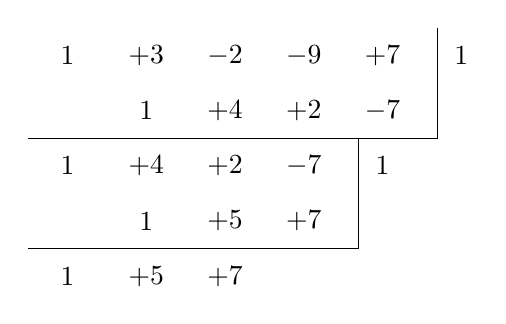
\begin{tikzpicture}[yscale=.7]
\foreach \x/\y in {1/1,2/+3,3/-2,4/-9,5/+7, 6/1}
{
    \node at (\x,3){$\y$};
}
\foreach \x/\y in {2/1,3/+4, 4/+2, 5/-7}
{
    \node at (\x,2){$\y$};
}
\foreach \x/\y in {1/1,2/+4,3/+2, 4/-7, 5/1}
{
    \node at (\x,1){$\y$};
}
\foreach \x/\y in {2/1,3/+5, 4/+7}
{
    \node at (\x,0){$\y$};
}
\foreach \x/\y in {1/1,2/+5,3/+7}
{
    \node at (\x,-1){$\y$};
}
\draw(.5,1.5)--(5.7,1.5)--(5.7,3.5);
\draw(.5,-.5)--(4.7,-.5)--(4.7,1.5);
% \draw(3.5,1.5)--(3.5,.5)--(4.7,.5);
\end{tikzpicture}
\end{center}

(说明:这里第一次除以$x-1$,所得商式的系数$1,4,2,-7$的和又为0,可知1又是方程$x^3+4x^2+2x-7=0$的根,所以利用综合除法,再将商式除以$x-1$,得到$x^2+5x+7$)\footnote{实际解题时,括号中的说明都可以省去.}.即
\[f(x)=(x-1)^2(x^2+5x+7)=0\]

这时商式$x^2+5x+7$已降为二次式了,解方程$x^2+5x+7=0$,得原方程的另外两个根
\[x=\frac{-5\pm\sqrt{3}i}{2}\]

由定理2,原方程有且仅有四个根.从而原方程在复数集$\mathbb{C}$中的解集是
\[\left\{1_{(2)}, \;\frac{-5+\sqrt{3}i}{2},\; \frac{-5-\sqrt{3}i}{2} \right\}\]
\end{solution}

由第9.5节的定理2及其推论,我们还可以得到:

\begin{thm}{定理3}
    如果既约分数$\frac{q}{p}$是整系数一元$n$次方程
\[a_nx^n+a_{n-1}x^{n-1}+\cdots +a_1x+a0=0\]
的根,那么$p$一定是$a_n$的约数,$q$一定是$a_0$的约数.
\end{thm}

\begin{thm}
 {推论1} 如果整系数一元$n$次方程的首项系数是1,那么这个方程的有理数根只可能是整数.   
\end{thm}

\begin{thm}
{推论2} 如果整系数一元$n$次方程有整数根,那么它一定是常数项的约数.    
\end{thm}

\begin{example}
    求方程$f(x)=2x^6+x^5-16x^4-6x^3+25x^2+20x+4=0$在复数集$\mathbb{C}$中的解集.
\end{example}

\begin{solution}
    原方程是一个整系数一元六次方程.由定理3,如果它有有理数根,只可能是:$\pm 1$, $\pm2$, $\pm4$, $\pm\frac{1}{2}$. 因为它的系数之和不为0,可知1不是它的根.利用综合除法,得
 \begin{center}
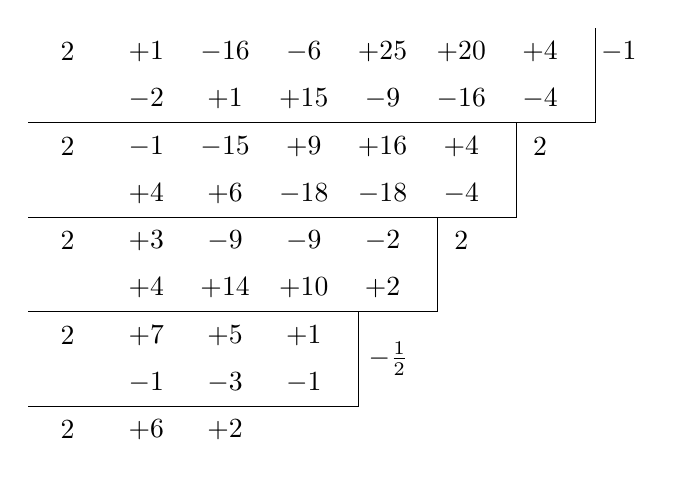
\begin{tikzpicture}[yscale=.6]
\foreach \x/\y in {1/2,2/+1,3/-16,4/-6,5/+25, 6/+20, 7/+4, 8/-1}
{
    \node at (\x,3){$\y$};
}
\foreach \x/\y in {2/-2,3/+1, 4/+15, 5/-9, 6/-16, 7/-4}
{
    \node at (\x,2){$\y$};
}
\foreach \x/\y in {1/2,2/-1,3/-15, 4/+9, 5/+16, 6/+4, 7/2}
{
    \node at (\x,1){$\y$};
}
\foreach \x/\y in {2/+4,3/+6, 4/-18, 5/-18, 6/-4}
{
    \node at (\x,0){$\y$};
}
\foreach \x/\y in {1/2,2/+3,3/-9,  4/-9, 5/-2, 6/2}
{
    \node at (\x,-1){$\y$};
}
\foreach \x/\y in {2/+4,3/+14, 4/+10, 5/+2}
{
    \node at (\x,-2){$\y$};
}
\foreach \x/\y in {1/2, 2/+7,3/+5, 4/+1}
{
    \node at (\x,-3){$\y$};
}
\foreach \x/\y in {2/-1,3/-3,  4/-1}
{
    \node at (\x,-4){$\y$};
}
\foreach \x/\y in {1/2,2/+6,3/+2}
{
    \node at (\x,-5){$\y$};
}

\draw(.5,1.5)--(7.7,1.5)--(7.7,3.5);
\draw(.5,-.5)--(6.7,-.5)--(6.7,1.5);
\draw(.5,-2.5)--(5.7,-2.5)--(5.7,-.5);
\draw(.5,-4.5)--(4.7,-4.5)--node[right]{$-\frac{1}{2}$}(4.7,-2.5);
\end{tikzpicture}
\end{center}

(说明:这里先除以$x+1$,得商式$2x^5-x^4-15x^3+9x^2+16x+4$,余数为0.方程$2x^5-x^4-15x^3+9x^2+16x+4=0$的有理数根只可能是$-1$,$\pm 2$, $\pm4$, $\pm\frac{1}{2}$.用心算可知$-1$不是它的根. 用综合除法除以$x-2$后,得商式$2x^4+3x^3-9x^2-9x-2$,
余数为0.方程$2x^4+3x^3-9x^2-9x-2=0$的有理数根只可能是$\pm 2$, $\pm\frac{1}{2}$. 用综合除法除以$x-2$后,得商式$2x^3+7x^2+5x+1$,余数为0.方程$2x^3+7x^2+5x+1=0$的系数都是正数,所以它没有正数根,它的有理数根只可能是$-\frac{1}{2}$. 用综合除法除以$x+\frac{1}{2}$后,得商式$2x^2+6x+2$,余数为0. $2x^2+6x+2$已经是二次式了.)即
\[f(x)=(x+1)(x-2)^2\left(x+\frac{1}{2}\right)(2x^2+6x+2)=0\]

解方程$2x^2+6x+2=0$,得原方程的另外两个根
\[x=\frac{-3\pm\sqrt{5}}{2}\]
从而原方程在复数集$\mathbb{C}$中的解集是
\[\left\{-1,\; 2_{(2)},\; -\frac{1}{2},\; \frac{-3+\sqrt{5}}{2},\; \frac{-3-\sqrt{5}}{2}\right\}\]
\end{solution}

\begin{example}
    求最简整系数方程(就是求一个整系数方程,并使最高次项系数取尽可能小的自然数)$f(x)=0$,已知它在复数集$\mathbb{C}$中的解集为$\left\{\frac{1}{2}_{(2)},\; i,\; -i\right\}$.
\end{example}

\begin{solution}
设所求的方程是
\[a\left(x-\frac{1}{2}\right)^2(x-i)(x+i)=0\quad (a\in\N, \text{ 且 } a\ne 0)\]
即
\[a\left(x^2-x+\frac{1}{4}\right)(x^2+1)=0\]

因为要求上式具有最简单的整系数,所以取$a=4$. 代入上式,得
\[4\left(x^2-x+\frac{1}{4}\right)(x^2+1)=0\]
即
\[\polynomial[reciprocal]{4,-4,5,-4,1}=0\]
\end{solution}

\begin{ex}
\begin{enumerate}
    \item (口答)在复数集$\mathbb{C}$中,下列方程有且仅有多少个根?
\begin{multicols}{2}
   \begin{enumerate}[(1)]
    \item $x^4+ 3x^2+ 4x+ 5= 0$
    \item $x^7= 1$
    \item $( x+ 1) ^{4}- ( x- 1) ^{4}= 0$
    \item $(x-1)^{2}(x-2)^{3}(x+3)^{4}=0$
\end{enumerate} 
\end{multicols}

\item \begin{enumerate}[(1)]
    \item 用综合除法验证 3是方程 $2x^3-5x^2-9x+18=0$ 的一个根;
    \item 把方程$2x^3-5x^2-9x+18=0$ 先化成
    $(x-x_{1})(ax^{2}+bx+c)=0$
    的形式,再化成
    $a(x-x_{1})(x-x_{2})(x-x_{3})=0$
    的形式.
\end{enumerate}
\item 求下列方程在复数集$\mathbb{C}$中的解集:
\begin{enumerate}[(1)]
    \item $3x^{3}- 11x^{2}+ 5x+ 3= 0$
    \item $6x^{4}+31x^{3}+25x^{2}-39x+9=0$
    \item $3x^{5}+4x^{4}-10x^{3}-14x^{2}+3x+6=0$
\end{enumerate}

\item 求最简整系数方程 $f(x)=0$, 已知它在复数集$\mathbb{C}$ 中的解集是:
\begin{multicols}{2}
\begin{enumerate}[(1)]
    \item $\left\{-1,-2,3\right\}$
    \item $\left\{-\frac{1}{2},\frac{2}{3},1\right\}$
    \item $\{-2,2_{(2)}\}$
    \item $\left\{1+i, 1-i, -\frac{\sqrt{3}}{2}, \frac{\sqrt{3}}{2}\right\}$
\end{enumerate}
\end{multicols}

\end{enumerate}
\end{ex}

\section{一元$n$次方程的根与系数的关系}
我们知道,如果一元二次方程
$ax^2+bx+c=0$
的两个根是$x_1,x_2$,那么根与系数之间有下列关系:
\[\begin{cases}
    x_1+x_2=-\frac{b}{a}\\
    x_1x_2=\frac{c}{a}
\end{cases}\]

一般地说,我们有如下的定理\footnote{此定理又叫韦达定理。韦达(Franciscus Vi\`{e}ta, 1540—1603),法国数学家.}:

\begin{thm}{定理}
如果一元$n$次方程$a_nx^n+a_{n-1}x^{n-1}+\cdots+a_1 x+a_0=0$在复数集$\mathbb{C}$中的根是$x_1,x_2,\ldots, x_n$,那么
\begin{equation}
\begin{cases}
x_1+x_2+\cdots+x_n=-\frac{a_{n-1}}{a_n}\\
x_1x_2+x_1x_3+\cdots+x_{n-1}x_n=\frac{a_{n-2}}{a_n}\\
x_1x_2x_3+x_1x_2x_4+\cdots+x_{n-2}x_{n-1}x_n=-\frac{a_{n-3}}{a_n}\\
\cdots\cdots\cdots\cdots\\
x_1x_2\cdots x_n=(-1)^n \frac{a_0}{a_n}
\end{cases}    \tag{*}
\end{equation}
\end{thm}

例如:当$n=3$时,有
\[\begin{cases}
    x_1+x_2+x_3=-\frac{a_2}{a_3}\\
    x_1x_2+x_1x_3+x_2x_3=\frac{a_1}{a_3}\\
    x_1x_2x_3=-\frac{a_0}{a_3}\\
\end{cases}\]
下面我们证明上述定理.

\begin{proof}
因为方程$a_nx^n+a_{n-1}x^{n-1}+\cdots +a_1x+a_0=0$的根是$x_1,x_2,\ldots ,x_n$.由上节定理1,可以把$f(x)=a_nx^n+a_{n-1}x^{n-1}+\cdots +a_1x+a_0$分解成$n$个一次因式与$a_n$的积:
\begin{equation}
    a_nx^n+a_{n-1}x^{n-1}+\cdots +a_1x+a_0=a_n(x-x_1)(x-x_2)\cdots (x-x_n) \tag{1}
\end{equation}

因为
\[\begin{split}
    (x-x_1)(x-x_2)\cdots (x-x_n) &=x^n-(x_1+x_2+\cdots +x_n)x^{n-1}\\
    &\qquad +(x_1x_2+x_1x_3+\cdots +x_{n-1}x_n)x^{n-2}\\
    &\qquad +\cdots +(-1)^n x_1x_2\cdots x_n
\end{split}\]
代入上面(1)式后,把每一项与$a_n$相乘,并将等号左边的多项式减去等号右边的多项式,所得的差$F(x)$是一个零多项式. 对$F(x)$进行整理,可知
\[\begin{split}
  F(x)&=[a_{n-1}+a_n(x_1+x_2+\cdots +x_n)]x^{n-1}\\
  &\qquad +\left[a_{n-2}-a_n(x_1x_2+x_1x_3+\cdots +x_{n-1}x_n)\right]x^{n-2}\\
  &\qquad +\cdots +\left[a_0-(-1)^n a_n x_1x_2\cdots x_n\right]
\end{split}\]

根据零多项式的定义,$F(x)$的系数都是0,所以   
\[\begin{cases}
    a_{n-1}+a_n(x_1+x_2+\cdots +x_n)=0\\
    a_{n-2}-a_n(x_1x_2+x_1x_3+\cdots +x_{n-1}x_n)=0\\
    \cdots \cdots \cdots \cdots \\
    a_0-(-1)^n a_n x_1x_2\cdots x_n=0
\end{cases}\]
由此即得
\[\begin{cases}
    x_1+x_2+\cdots +x_n=-\frac{a_{n-1}}{a_n}\\
   x_1x_2+x_1x_3+\cdots +x_{n-1}x_n=\frac{a_{n-2}}{a_n}\\
   \cdots \cdots \cdots \cdots \\
    x_1x_2\cdots x_n=(-1)^n \frac{a_{0}}{a_n}
\end{cases}\]
\end{proof}

这个定理的逆命题也成立,即对于任何一元$n$次方程
\begin{equation}
f(x)=a_nx^n+a_{n-1}x^{n-1}+\cdots +a_1x+a_0=0 \tag{*}
\end{equation}
如果有$n$个数$x_1,x_2,\ldots,x_n$满足(*)式,那么$x_1,x_2,\ldots,x_n$一定是方程$f(x)=0$的根.

\begin{example}
    已知方程$2x^3-5x^2-4x+12=0$有2重根,利用一元$n$次方程的根与系数的关系,求这个方程在复数集$\mathbb{C}$中的解集.
\end{example}

\begin{solution}
设原方程在$\mathbb{C}$中的解集为$\{\alpha_{(2)},\beta\}$,那么
\[\begin{cases}
    2\alpha +\beta =\frac{2}{5} & (1)\\
    \alpha^2 +2\alpha \beta =-2 & (2)\\
    \alpha^2 \beta =-6 & (3)\\
\end{cases}\]
(说明:这里有两个未知数、三个方程.我们可以选其中两个方程,求出满足这两个方程的,再代入另一个方程,如能满足,就是方程组的解,否则不是.)解(1),(2)两式组成的方程组,得
\[\begin{cases}
    \alpha=2\\ \beta =-\frac{3}{2}
\end{cases},\quad \text{或} \quad \begin{cases}
    \alpha=-\frac{1}{3}\\[1ex] \beta=\frac{19}{6}
\end{cases}\]

第一个解满足(3)式;第二个解不满足(3)式,应舍去. 所以原方程在$\mathbb{C}$中的解集为$\left\{2_{(2)},-\frac{3}{2}\right\}$.
\end{solution}

\begin{example}
    当且仅当$k$是什么数的时候,方程$x^3-6x^2+3x+k=0$的三个根成等差数列\footnote{本书中涉及等差、等比数列的问题,都限于在实数集内讨论.}?
\end{example}

\begin{solution}
设原方程在$\mathbb{C}$中的三个根成等差数列,并分别记作$a-d$, $a$, $a+d\; (d\ge 0)$,那么
\[\begin{cases}
    (a-d)+a+(a+d)=6\\
    a(a-d)+a(a+d)+(a+d)(a-d)=3\\
    a(a-d)(a+d)=-k
\end{cases}\]
整理后,得
\[\begin{cases}
    3a=6& (1)\\
    3a^2-d^2=3& (2)\\
    a^3-ad^2=-k & (3)\\
\end{cases}\]
由(1)式,得$a=2$;代入(2)式,得$d=3$; 再代入(3)式,便得
$k=10$.

这就是说,要使原方程的三个根成等差数列,$k$必须等于10.反过来,容易验证,当方程中的$k=10$时,$-1(=a-d)$,$2(=a)$,$5(=a+d)$三个数确实是原方程的根,且成等差数列. 所以当且仅当$k=10$时,原方程的三个根成等差数列.
\end{solution}

\begin{ex}
利用一元$n$次方程的根与系数的关系解下列各题:
\begin{enumerate}
\item 已知方程$6x^4+7x^3-36x^2-7x+6=0$的根中有三个是$-\frac{1}{2},\frac{1}{3},2$,求这个方程在复数集$\mathbb{C}$中的解集.
\item 已知方程$2x^3+x^2-8x-4=0$的根都是实数,且有两个互为相反数,求这个方程的解集.
\item 已知方程$x^3-9\sqrt{2}x^2+46x-30\sqrt{2}=0$的三个根成等差数列,求这个方程的解集.
\end{enumerate}
\end{ex}

\section{一元$n$次方程的根的基本对称函数}

上节韦达定理中出现的$x_1+x_2+\cdots +x_n$, $x_1x_2+x_1x_3+\cdots +x_{n-1}x_n$, $x_1x_2x_3+x_1x_2x_4+\cdots +x_{n-2}x_{n-1}x_n,\ldots,x_1x_2\cdots x_n$, 称作一元$n$次方程的根的基本对称函数. 为了书写简便,我们把前$n-1$个根的基本对称函数分别记作$\Sigma x_1$,$\Sigma x_1x_2,\ldots, \Sigma x_1x_2\cdots x_{n-1}$. 最后一个只有一项,不再用“$\Sigma$”. 于是有下列的性质:

\begin{enumerate}
    \item $\Sigma x_1x_2\cdots x_k$共有${\rm C}^k_n=\frac{n(n-1)\cdots (n-k+1)}{k(k-1)\cdots 2\cdot 1}$项.
    \item 令$S_1=\Sigma x_1$, $S_2=\Sigma x^2_1$, $S_3=\Sigma x^3_1,\ldots ,S_k=\Sigma x^k_1$,它们是一元$n$次方程的根的同次幂的和,也都是根的对称函数.
\end{enumerate}


设$x_1,x_2,\ldots ,x_n$是一元$n$次方程$f(x)=x^n+b_1x^{n-1}+b_2x^{n-2}+\cdots +b_{n-1}x+b_n=0$的$n$个根(最高次项系数为1),那么令$k=1,2,\ldots ,n-1$时,有
\[S_k+b_1S_{k-1}+b_2S_{k-2}+\cdots +b_{k-1}S_1+kb_k=0\]

当 $k\geqslant n$ 时,有 $S_k+b_1S_{k-1}+\cdots+b_nS_{k-n}=0$(这个公式叫
做牛顿公式,它可以利用多项式的导数加以证明)

\begin{example}
    求方程$x^3-2x^2+5x-3=0$的根的平方和,立方和
及四次幂的和.
\end{example}

\begin{solution}
    设方程根的平方和为$S_2$, 立方和为 $S_3$, 四次幂的和
为$S_{4}$

$\because\quad b_1=-2, \; b_2=5,\; b_3=-3$,由韦达定理可直接得出$S_{1}=2$. 利用牛顿公式,有
\[\begin{cases}
    S_{2}+ b_{1}S_{1}+ 2b_{2}= 0\\
    S_{3}+ b_{1}S_{2}+ b_{2}S_{1}+ 3b_{3}= 0\\
    S_4+ b_1S_3+ b_2S_2+ b_3S_1= 0
\end{cases}\Longrightarrow \begin{cases}
    S_{2}= - b_{1}S_{1}- 2b_{2}=2\times2-2\times5=-6\\
    S_3=- b_{1}S_{2}- b_{2}S_{1}- 3b_{3}
    =-13\\
    S_4= b_1S_3- b_2S_2- b_3S_1 =10
\end{cases}\]

$\therefore\quad $根的平方和为$-6$,立方和为$-13$. 
四次幂的和为10.
\end{solution}

\begin{rmk}
    对于高次(3 次以上)方程没有一般的求根方法。而牛顿公式告诉我们不必求方程的根,即可求出方程所有根的和、根的平方和,……,根的同次幂的和的方法.
\end{rmk}

\section{实系数方程虚根成对定理}

我们知道,如果 $\Delta=b^2-4ac<0$, 那么实系数一元二次方
程$ax^{2}+bx+c=0$ 有一对虚数根,它们互为共轭虚数,即
$$x=\frac{-b\pm\sqrt{4ac-b^{2}}i}{2a}$$

一般地说,关于实系数一元n次方程的虚数根,有下面的性质:

\begin{thm}
   {定理} 如果虚数$a+bi$是实系数一元$n$次方程$f(x)=0$的根,那么$a-bi$也是这个方程的根,并且它们的重数相等. 
\end{thm}

\begin{proof}
由$a+bi$是实系数一元$n$次方程$f(x)=0$的根,可知$f(a+bi)=0$. 我们先来证明也是方程$f(x)=0$的根,为此只需证明$f(a-bi)=0$.

考虑多项式
\begin{equation}
\begin{split}
    g(x)&=[x-(a+bi)][x-(a-bi)]\\
&=(x-a)^2-(bi)^2\\
&=x^2-2ax+(a^2+b^2)
\end{split}\tag{1}
\end{equation}
这是一个实系数二次三项式. 用$g(x)$除$f(x)$,设商式为$q(x)$,那么余式的次数不大于1,可以表示为$mx+n$(其中$m,n$为实数). 于是
\begin{equation}
    f(x)=g(x)\cdot q(x)+mx+n \tag{2}    
\end{equation}

把$x=a+bi$代入上式,左边$f(a+bi)=0$,又由(1)式知右边的$g(a+bi)=0$,从而右边的$m(a+bi)+n=0$,即
\[am+n+bmi=0\]

根据复数等于零的条件,得
\[am+n=0,\qquad bm=0\]
由于$b\ne 0$(否则$a+bi$不是虚数),所以$m=0$,由此$n=0$. 又由(1)式知$g(a-bi)=0$,所以由(2)式,
\[\begin{split}
    f(a-bi)&=g(a-bi)\cdot q(a-bi)+m(a-bi)+n\\
  &=0\cdot q(a-bi)+0\cdot (a-bi)+0=0.  
\end{split}\]
即$a-bi$是方程$f(x)=0$的根.

现在再证明$a+bi$与$a-bi$的重数相等,由上面的证明可
知$m=0$, $n=0$,代入(2)式,得
\[f(x)=g(x)\cdot q(x)\]
这说明$g(x)$整除$f(x)$. 因为$f(x)$, $g(x)$的系数都是实数,非零实系数多项式除以实系数多项式,商式仍然是实系数多项式,所以$q(x)$的系数也都是实数. 如果$a+bi$是方程$f(x)=0$的重根,那么它必然是方程$q(x)=0$的根,根据上面的证明,$a-bi$也必然是方程$q(x)=0$的根. 这样也是方程$f(x)=0$的重根. 设$a+bi$与分别是方程$f(x)=0$的$s$重根与$t$重根,重复运用这个推理方法,可知$s\le t$;同理可证$t\le s$. 所以$s=t$.
\end{proof}


由上面的定理可知,在实系数一元n次方程中,虚数根总是成对出现的.

\begin{example}
    求方程$2x^4-6x^3+21x^2+14x+39=0$在复数集$\mathbb{C}$中的解集,已知它的根中有一个是$2-3i$.
\end{example}

\begin{solution}
\textbf{解法一:} 这是一个一元四次方程,在复数集$\mathbb{C}$中有且仅有四个根. 因为它的系数都是实数,且是它的根,可知$2+3i$也是它的根.

把$2x^4-6x^3+21x^2+14x+39$除以
$[x-(2-3i)][x-(2+3i)]$, 
也就是除以$x^2-4x+13$,得商式$2x^2+2x+3$. 因此原方程可以化为
\[[x-(2-3i)][x-(2+3i)](2x^2+2x+3)=0\]

解方程$2x^2+2x+3=0$,得$x=\frac{-1\pm\sqrt{5}i}{2}$,所以原方程的解集是
\[\left\{2-3i,\; 2+3i,\; \frac{-1+\sqrt{5}i}{2},\; \frac{-1-\sqrt{5}i}{2}\right\}\]

\textbf{解法二:} 原方程有两个根$2-3i$, $2+3i$,设另外两个根为$\alpha, \beta$,由根与系数的关系,有
\[\begin{cases}
    \alpha+\beta+(2-3i)+(2+3i)=3\\
    \alpha\cdot \beta\cdot (2-3i)\cdot (2+3i)=\frac{39}{2}
\end{cases}\]
即
\[\begin{cases}
    \alpha+\beta=-1 \\ \alpha\beta=\frac{3}{2}
\end{cases}\]
所以$\alpha,\beta$是一元二次方程$2x^2+2x+3=0$的根. 解这个一元二次方程,得两个根$x=\frac{-1\pm\sqrt{5}i}{2}$. 从而原方程的解集是
\[\left\{2-3i,\; 2+3i,\; \frac{-1+\sqrt{5}i}{2},\; \frac{-1-\sqrt{5}i}{2}\right\}\]
\end{solution}

\begin{example}
    求次数最低的实系数方程
$f(x)=0$,已知它在复
数集$\mathbb{C}$中的解集含有$i$,$-1+i$,0
这三个数.
\end{example}

\begin{solution}
    根据实系数方程虚根成对定理,如果$i$,$-1+i$是所求实系数方程$f(x)=0$的根,那么它们的共轭虚数$-i$,$-1-i$也是这个方程的根,所以所求的实系数方程至少有五个根$\pm i$,$-1\pm i$,0,也就是说,$f(x)$至少有五个一次因式$x\mp i$, $x+1\mp i$,$x$,把$f(x)$写成这五个一次因式与一个常数$a\; (a\in\mathbb{C}, \text{ 且 } a\ne 0)$的积
\[f(x)=a(x-i)(x+i)(x+1-i)(x+1+i)x\]

取$a=1$,那么,实系数一元五次方程
\[(x-i)(x+i)(x+1-i)(x+1+i)x=0\]
即
\[x^5+2x^4+3x^3+2x^2+2x=0\]
就是所求的方程.
\end{solution}

\begin{ex}
\begin{enumerate}
    \item 已知方程$3x^4-2x^3+10x^2-2x+7=0$的根中有一个是$i$,求它在复数集$\mathbb{C}$中的解集.
    \item 求次数最低的实系数方程$f(x)=0$,已知它在复数集$\mathbb{C}$中的解集含有下列数:
\begin{multicols}{2}
\begin{enumerate}[(1)]
    \item $3+2i$
    \item $-2,\; 1-i$
\end{enumerate}
\end{multicols}
    \item 已知虚数$-1+\sqrt{2}i$是实系数方程$x^3+3x^2+ax+b=0$的根,求$a$,$b$的值以及这个方程在复数集$\mathbb{C}$中的解集.
\end{enumerate}
\end{ex}

\section{有理系数方程$f(x)=0$的有关无理根的定理}

\begin{thm}
{定理} 设$f(x)=0$是有理系数方程
\begin{enumerate}[(1)]
\item 若方程$f(x)=0$有无理根$a+b\sqrt{d}\; (a,b,d\in\Q,\; \sqrt{d}\in\overline{\Q} \text{ 且 } b\ne 0)$,则方程必还有另一个无理根$a-b\sqrt{d}$;
\item 若方程$f(x)=0$有无理根$a\sqrt{c}+b\sqrt{d}\; (a,b,c,d\in\Q,\; \sqrt{c},\sqrt{d}\in\overline{\Q}\text{ 且 }ab\ne 0)$,则方程必还有另外三个无理根:$a\sqrt{c}-b\sqrt{d}$, $-a\sqrt{c}+b\sqrt{d}$和$-a\sqrt{c}-b\sqrt{d}$;
\item 若$方程f(x)=0$有一个根是$a\sqrt{c} +bi\; (a,b,c\in\Q,\; \sqrt{c}\in\overline{\Q},\text{ 且 }ab\ne 0)$则方程必还有三个根:$a\sqrt{c}-bi$,$-a\sqrt{c}+bi$和$-a\sqrt{c}-bi$;
\item 若$方程f(x)=0$有一个根$a\sqrt{c}+b\sqrt{d}i\; (a,b,c,d\in\Q,\; \sqrt{c},\sqrt{d}\in\overline{\Q}\; \text{ 且 } ab\ne 0)$,则方程必还有三个根:$a\sqrt{c}-b\sqrt{d}i$, $-a\sqrt{c}+b\sqrt{d}i$和$-a\sqrt{c}-b\sqrt{d}i$.    
\end{enumerate}

\end{thm}

\begin{example}
求作含有根$\sqrt{3}+i$和$1-\sqrt{3}i$的次数最低的最简
有理系数的整式方程.
\end{example}

\begin{solution}
\textbf{解法一:} 由上述两个定理可知,方程有以下 6 个根:
$1\pm\sqrt{3}i$, $\sqrt{3}\pm i$ 和$-\sqrt3\pm i$
故所求的方程应为    
\[\begin{split}
    [x-(1+\sqrt{3}i)]&\cdot [x-(1-\sqrt{3}i)]\cdot [x-(\sqrt{3}+i)]\cdot\left[x-(\sqrt{3}-i)\right]\\
&\cdot \left[x-(-\sqrt{3}+i)\right]\cdot\left[x-(-\sqrt{3}-i)\right]=0\\
\end{split}\]
化简, 即为$x^6-2x^5+8x^3-32x+64=0$

\textbf{解法二:}先作含根$\sqrt{3}+i$的次数最低的有理系数的最
简整式方程,它有四个根,所以是四次方程

设 $x= \sqrt {3}+i$, 则$x-i=\sqrt{3}$

$\therefore\quad (x-i)^2=3$,即$x^2-2ix-4=0$

$\therefore\quad x^2-4=2ix \Longrightarrow (x^2-4)^2=(2ix)^2$

即$x^4-4x^2+16=0$

再作含根$1-\sqrt{3}i$的最简有理系数方程,该方程有两个
根,所以是二次方程。

设 $x= 1- \sqrt {3}i$, 则$x-1=-\sqrt{3}i$

$\therefore\quad (x-1)^2=(-\sqrt{3}i)^2$


化简,即 $x^2-2x+4=0$. 故所求的方程是
$$(x^4-4x^2+16)(x^2-2x+4)=0$$
即$$x^6-2x^5+8x^3-32x+64=0$$
\end{solution}

\section*{习题二}
\begin{enumerate}
    \item 求证任何复条数一元$n$次方程都可化为$x^{n}+b_{x-1}x^{n-1}+\cdots+b_{1}x+b_{0}=0$的形式,其中$b_0,b_1,\ldots,b_{n-1}\in \mathbb{C}$.
    \item 求下列方程在复数集$\mathbb{C}$中的解集:
\begin{enumerate}[(1)]
    \item $x^{3}-8x^{2}+20x-16=0$ 
    \item $x^4+ x^3- 5x^2+ x- 6= 0$ 
    \item $ 2x^4+ 9x^3- 27x^2+ 53x- 21= 0$ 
    \item $5x^{4}+6x^{3}-5x-6=0$
\end{enumerate}

\item 求最简整系数方程 $f(x)=0$, 已知它在复数集$\mathbb{C}$ 中的解集是:
\begin{multicols}{2}
\begin{enumerate}[(1)]
    \item $\left\{0, 2- \sqrt {3}, 2+ \sqrt {3}, 2i, - 2i\right\}$
    \item $\left\{\frac12_{(2)},-\frac23_{(3)}\right\}$
\end{enumerate}    
\end{multicols}

\item 求证:
\begin{enumerate}[(1)]
\item 如果一元$n$次方程 $f(x)=0$ 各项的余数都是正数,那
么它没有正数根;
\item 如果一元$n$次方程$f(x)=0$各奇次项的条数都是正
数,各偶次项(包括常数项$a_0$)的系数都是负数,那么它
没有负数根;
\item 方程$2x^6+3x^4+5x^2+7=0$ 没有实数根。
\end{enumerate}

\item 利用第 4 题的结论,求下列方程在复数集$\mathbb{C}$中的解集:
\begin{multicols}{2}
\begin{enumerate}[(1)]
    \item $ x^{3}+ \frac 72x^{2}+ \frac 52x+ \frac 12= 0$ 
    \item $x^3-\frac23x^2+3x-2=0$
\end{enumerate}    
\end{multicols}

利用一元$n$次方程根与系数的关系解下列各题(第6—9
题):

\item \begin{enumerate}[(1)]
    \item 已知方程 $18x^3+9x^2-74x+40=0$ 的根中有一个是另一个的 2倍,求这个方程在复数集$\mathbb{C}$中的解集;
    \item 已知方程 $x^4+4x^3+10x^2+12x+9=0$ 在复数集$\mathbb{C}$中
    的四个根是 2 重根$a$, 2重根$b$. 求$a,b$的值.
\end{enumerate}

\item \begin{enumerate}[(1)]
\item 已知方程$x^4-4x^3-34x^2+ax+b=0$的四个根成等差
    数列,求$a,b$的值,并且求这个方程的解集;
    \item 已知方程 $8x^3-14x^2+kx+27=0$ 的三个根成等比数
    列,求$k$的值,并且求这个方程的解集。
\end{enumerate}

\item 已知方程 $x^3+px^2+qx+r=0\; (p,q,r\in \mathbb{C})$在复数集$\mathbb{C}$中的根是 $x_1,x_2,x_3$, 求下列各式的值:
\begin{multicols}{2}
\begin{enumerate}[(1)]
    \item $\frac{1}{x_1x_2}+\frac{1}{x_1x_3}+\frac{1}{x_2x_3}$
    \item $\frac{1}{x_1}+\frac{1}{x_2}+\frac{1}{x_3}$
    \item $x_1^2+x_2^2+x_3^2$
    \item $x_1^2x_2^2+x_1^2x_3^2+x_2^2x_3^2$
\end{enumerate}
\end{multicols}
    
\item 设方程$x^3+2x^2-x+3=0$在复数集$\mathbb{C}$中的根是$x_1,x_2,x_3$, 求一元三次方程,使它在$\mathbb{C}$中的根是:
\begin{multicols}{3}
\begin{enumerate}[(1)]
    \item $2x_1,\; 2x_2,\; 2x_3$
    \item $-x_1,\; -x_2,\; -x_3$
    \item $\frac{1}{x_{1}},\; \frac{1}{x_{2}},\; \frac{1}{x_{3}}$
\end{enumerate}
\end{multicols}

\item 根据已知条件,求下列方程在复数集$\mathbb{C}$中的解集:
\begin{enumerate}[(1)]
\item $x^4-3x^3+10x^2+42x-20=0$, 已知它的根中有一个
    是 $3+i$ 
    \item $x^4-3x^3+5x^2+4x+2=0$, 已知它的根中有一个是
    $i- 1$
    \item $x^{4}-4x^{3}+11x^{2}-14x+10=0$, 已知它的根中有两个
    是 $a+bi$, $a+2bi$, 其中 $a,b\in \R$, 且 $b\neq0$
\end{enumerate}

\item 求次数最低的实系数方程$f(x)=0$,已知它在复数集$\mathbb{C}$中的解集含有下列数:
\begin{multicols}{2}
\begin{enumerate}[(1)]
    \item $1,\; \frac{-1+\sqrt{3}i}{2}$
    \item $2+i,\; -1+i$
    \item $\pm 1,\; i$
    \item $\sqrt{2},\; \sqrt{2}i$
\end{enumerate}
\end{multicols}

\item 求证实系数一元$n$次方程在$n$为奇数时,有奇数个实根;在$n$为偶数时,有偶数个实根,或者没有实根.
\item 已知虚数$a+bi\; (a,b\in\R)$ 是实系数方程的$x^3+px+q=0$的根,求证$2a$是方程$x^3+px-q=0$的根.
\item 一个长方体的长、宽、高分别是12cm,5cm,6cm.要使各度(即长、宽、高)都增加一个相同的长度,体积增加186${\rm cm}^3$,这个增加的长度应是多少?
\item 把边长为6dm的正方形铁板的四角各截去一个相同的小正方形,然后把各边折起来做成一个无盖的长方体盒. 已知这个长方体盒的容积(铁板厚度不计)是16${\rm dm}^3$,求截去的小正方形每边的长.
\end{enumerate}

\section{本章小结}

\subsection*{知识结构分析}

\begin{enumerate}
    \item 复系数一元$n$次多项式及有关概念
\begin{enumerate}[(1)]
    \item 复系数一元$n$次多项式的标准形式是
    $$a_nx^n+a_{n-1}x^{n-1}+\cdots+a_1x+a_0$$ 其中$a_n\ne 0$, $a_k$为复数$(k=0,1,\ldots ,n)$. 根据需要,该多项式也常常看作是定义在复数集$\mathbb{C}$上的函数,并记作$f(x)$, $g(x)$等.
    \item 零次多项式与零多项式
    
单独一个非零复数,可看作零次多项式;系数都是零的多项式称作零多项式. 显然对于$\mathbb{C}$上的每一个$x$值,零多项式的值恒为零.
\end{enumerate}

\item 余数定理和因式定理

多项式$f(x)$除以$x-b\; (b\in\mathbb{C})$所得的余数为$f(b)$. 余数定理的一个重要推论是多项式$f(x)$有一个因式$x-b$的充要条件是$f(b)=0$,此即因式定理.

\item 任何一个复系数一元$n$次多项式$f(x)$有唯一确定的因式分解形式:
\[f(x)=a_n(x-x_1)^{k_1}(x-x_2)^{k_2}\cdots (x-x_m)^{k_m}\]
其中$k_1,k_2,\ldots,k_m\in\N$,且$k_1+k_2+\cdots+k_m=n$,复数$x_1,x_2,\ldots,x_m$互不相等,$x-x_i\; (i=1,2,\ldots,m)$叫做多项式$f(x)$的$k_i$重因式.

此即多项式因式分解唯一性定理. 这里不考虑各个一次因式的书写顺序及常数因子.

\item 若整系数多项式$f(x)=a_nx^n+a_{n-1}x^{n-1}+\cdots+a_1x+a_0$有因式$x-\frac{q}{p}$($p,q$为互质的整数),则$p$一定是$a_n$的约数,$q$一定是$a_0$的约数.由此我们可借助综合除法,求出整系数多项式的整系数一次因式,或可以证明它没有这个因式.
\item 多项式因式分解与解方程密切相关.如果$x-x_i\; (i=1,,2,\ldots,m)$是多项式$f(x)$的$k_i$重因式,那么$x_i$叫做方程$f(x)=0$的$k_i$重根. 由此可得出“复系数一元$n$次方程在复数集$\mathbb{C}$中有且仅有$n$个根($k$重根算作$k$个根)”. 这个重要定理揭示出复系数一元$n$次方程在$\mathbb{C}$中根的个数.

显然实系数一元$n$次方程在$\R$中的根没有这个性质.
\item 韦达定理给出了复系数一元$n$次方程的根与其系数的关系,即$x_1,x_2,\ldots,x_n$是复系数一元$n$次方程$f(x)=0$的根,则有
\[\begin{cases}
x_1+x_2+\cdots+x_n=-\frac{a_{n-1}}{a_n}\\
x_1x_2+x_1x_3+\cdots+x_{n-1}x_n=\frac{a_{n-2}}{a_n}\\
x_1x_2x_3+x_1x_2x_4+\cdots+x_{n-2}x_{n-1}x_n=-\frac{a_{n-3}}{a_n}\\
\cdots\cdots\cdots\cdots\\
x_1x_2\cdots x_n=(-1)^n \frac{a_0}{a_n}
\end{cases} \]
其逆定理也是成立的.

\item 实系数一元$n$次方程的虚根成对出现定理,揭示了实系数一元$n$次方程的根的特点,与此类似的是,有理系数一元$n$次方程的无理根$a+b\sqrt{c}$或$a\sqrt{c}+b\sqrt{d}$(其中$a,b,c,d\in\Q$, $\sqrt{c},\sqrt{d}\in\overline{\Q}$)也是成对出现的.

由此可在解方程的过程中,根据方程的条件选择较简便的方法,如首先用综合除法求出有理根,再根据若$a+bi\; (a,b\in\R)$是实系数方程$f(x)=0$的根. 便可知$(x-a-bi)(x-a+bi)$必为$f(x)$的两个因式. 从而可降低方程$f(x)=0$的次数.
\end{enumerate}

\subsection*{几点说明}
\begin{enumerate}
    \item 零多项式的定义是用“待定系数法”确定多项式的理论依据:即两个一元同次多项式恒等的充要条件是对应项(次
    数相同的项)系数相等.
    \item 综合除法是求一元$n$次多项式$f(x)$的“$x-b$”型(或$x-\frac{q}{p}$,$p,q$互质)因式的简便方法. 简便之处在于只是利用了它的系数就解决了问题.
    
    它是通过竖式除法分离系数,改变运算程序得出来的.它提示我们去探求其它运算问题,以简化运算过程和改变运算程序,提高运算速度的途径.
    \item 易混淆的概念,如零次多项式与零多项,要给予足够的重视.
    \item 应用定理时,定理的条件不能忽视.如方程$x^3+2x^2-3x+2-4i=0$有一根为$i$时,误认为$-i$也是方程的根.
    \item 运用综合除法时,对所缺的项应予以补零.否则将导致错误.
    \item 韦达定理本身并不能帮助我们直接解方程,但是已知方程的一部分根,或方程的根之间的某些关系时,用韦达定理可列出方程(组),解这个方程(组). 可求得方程的其余根或全部根.
    
    利用韦达定理,可以不解方程而求出根的对称式的值. 
    
    利用韦达定理还可以求出以已知数为根的方程.
\end{enumerate}


\section*{复习题九}
\begin{center}
    \bfseries A
\end{center}

\begin{enumerate}
    \item 计算$(5x^2-2x^3+6x^4-18)\div(2x^2+1)$, 并把结果写成
    “$f(x)=g(x)q(x)+r(x)$”的形式。
    \item 一个多项式除法的除式是 $2x^2+3x-5$, 商式是 $3x-5$,余
    式是$-7$,求被除式。
    \item 用综合除法求商式及余数。其中哪些能够整除,哪些不能整除?
\begin{multicols}{2}
\begin{enumerate}[(1)]
\item $( a^{3}- b^{3}) \div ( a- b) $
\item $( a^{4}- b^{4}) \div ( a- b)$  
\item $( x^{6}- y^{6}) \div ( x+ y)$ 
\item  $( x^{5}+ y^{5}) \div ( x+ y)$ 
\item $( m^{5}- n^{5}) \div ( m+ n) $ 
\item $( m^{6}+ n^{6}) \div ( m- n)$  
\item $( u^{6}+ v^{6}) \div ( u+ v)$  
\item $( u^{7}+ v^{7}) \div ( u- v) $
\end{enumerate}
\end{multicols}

    \item 用综合除法求商式及余数:
\begin{enumerate}[(1)]
\item  $( 2x^{3}- 3x^{2}+ 8x- 12) \div ( 2x- 3)$ 
\item $( 4a^{3}+ 2a^{2}b- 8ab^{2}- 12b^{3}) \div ( 2a+ 3b)$ 
\item $( 3x^{4}+ 2x^{2}- 5x) \div ( 3x- 1)$ 
\item  $( 3x^{4}- 2x^{3}y+ 3x^{2}y^{2}- 2xy^{3}+ 3y^{4}) \div ( 3x+ 2y)$
\end{enumerate}

    \item \begin{enumerate}[(1)]
    \item 设 $f(x)=x^n+a^n$(其中$n\in \N$), 求$f(x)$除以$x-a$ 所
    得的余式,又求$f(x)$除以$x+a$所得的余式
    \item 设 $f(x)=x^n-a^n$(其中$n\in \N$), 求 $f(x)$除以$x-a$ 所得
    的余式,又求$f(x)$除以$x+a$所得的余式
    \item 通过第(1),(2)小题,说出在什么情况下,$x^n+a^n$或
    $x^n-a^n$(其中$n\in \N$)有因式 $x-a$ 或 $x+a$
    \end{enumerate}

\item 求证$x^3-4ax^2-10bx+16$有因式$x+2$的充要条件是
$a=\frac{1}{4}(2+5b)$
\item 把下列多项式分解因式:
\begin{enumerate}[(1)]
\item $y^{4}+ 5y^{3}+ 22y^{2}+ 80y+ 96$ 
\item $a^{4}- 4a^{3}b- 7a^{2}b^{2}+ 22ab^{3}+ 24b^{4}$ 
\end{enumerate}

\item 在复数集$\mathbb{C}$中解下列方程或方程组。
\begin{enumerate}[(1)]
    \item $x^{3}+ \frac 72x^{2}- 1= 0$ 
    \item $4x^{4}+ 7x^{3}- 22x^{2}- 35x+ 10= 0$
    \item $5x^{4}- 29x^{3}+ 14x^{2}- 116x- 24= 0$
    \item $x^{4}- x^{3}+ \frac 14x^{2}- 4x- 15= 0$
    \item $\begin{cases} x^3+ y^3= 19 \\ y= 2x+ 7  \end{cases}$
    \item $\begin{cases}x^{2}+y^{2}=52\\y=x^{2}-11x+34\end{cases}$
\end{enumerate}

\item \begin{enumerate}[(1)]
\item 已知方程$x^4-x^3+mx^2+nx-6=0$在复数集$\mathbb{C}$中有两
个根的和为 3,积为 2,求$m,n$的值,并且求方程在$\mathbb{C}$中
的解集;
\item 已知方程 $x^3+3x^2+mx+n=0$ 的三个根成等差数列,
方程$x^3-(m-2)x^2+(n-3)x-8=0$的三个根成等比
数列,求$m,n$的值。
\end{enumerate}

\item 设方程$2x^3-4x^2+x-6=0$在复数集$\mathbb{C}$中的根是$x_1,x_2,x_3$, 求在$\mathbb{C}$中的根是 $x_1+1,x_2+1,x_3+1$ 的一元三次方
程。
\item 已知方程$f(x)=2x^4-3x^3+ax^2+bx+c=0$在复数集$\mathbb{C}$
中有3重根$-1$,另一个根是$x_4$,求$a,b,c,x_4$的值.
\item 求方程$x^3+ix^2-4x-4i=0$在复数集$\mathbb{C}$中的解集.
\item 已知方程$x^3+2x^2-3x+2-4i=0$的根中有一个是$-i$,求这个方程在复数集$\mathbb{C}$中的解集.
\item 已知方程$x^3-9x^2+33x-65=0$的根中有一个虚根的模等于$\sqrt{13}$,求这个方程在复数集$\mathbb{C}$中的解集.
\item 一个长方体的长是宽的2倍,高比宽少2厘米,它的体积是490厘米$^3$,求它的长、宽、高.
\item 某厂一种轻工产品第一年的产值为200万元,以后三年逐年按同样的百分数递增,四年的总产值为928.2万元,求产值每年比上一年增加的百分数.
\end{enumerate}

\begin{center}
    \bfseries B
\end{center}
\begin{enumerate}\setcounter{enumi}{16}
\item 用综合除法求$(a^3-b^3+c^3+3abc)\div (a-b+c)$的商式及余数.
\item \begin{enumerate}[(1)]
\item 证明$x^3+y^3+z^3-3xyz$有因式$x+y+z$,并把它分解因式.
\item 利用第(1)小题的结果把下列各式分解因式:
\begin{enumerate}[(i)]
    \item $a^3-b^3+c^3+3abc$;
    \item $8a^3+b^3+c^3-6abc$.
\end{enumerate}
\end{enumerate}

\item \begin{enumerate}[(1)]
\item 证明$a(b-c)^3+b(c-a)^3+c(a-b)^3$有因式$a-b$, $b-c$, $c-a$,并把它分解因式;
\item 证明$(ay+bx)^3+(ax+by)^3-(a^3+b^3)(x^3+y^3)$有因式$x+y$,也有因式$a+b$,并把它分解因式.
\end{enumerate} 

\item 把$y^7+2y^6-y^5-2y^4+4y^3+8y^2-4y-8$分解因式.
\item 已知$x^4+ax^3-4x^2+bx-12$有因式$x-2$,又有因式$x+3$,确定$a,b$的值,并把这个多项式分解因式.

\item 已知$x^4+4x^{2}+ax+b$有一个因式$x^2+x+1$, 求$ a,b$的值,并把这个多项式分解因式。
\item 已知多项式$f(x)$除以$x+2$所得的余数为 1, 除以$x+3$ 所得的余数为$-1$. 求 $f(x)$除以$(x+2)(x+3)$所得的余式.
\item 求证多项式 $f(x)$除以$(x-a)(x-b)$(其中 $a\neq b$)所得的
余式是
$$\frac{f(a)-f(b)}{a-b}x+\frac{af(b)-bf(a)}{a-b}$$
\item 设方程$x^3-x^2+3x-2=0$在复数集$\mathbb{C}$中的根是$x_1,x_2,x_3$
\begin{enumerate}[(1)]
\item 求证$x_{1},x_{2},x_{3}$都不是有理数;
\item 求证$x_{1},x_{2},x_{3}$中有两个是虚数(提示:先求出$x_1^{2}+x_{2}^{2}+x_3^2$的值);
\item 求证对任何实数$k$, 方程$x^3-x^2+3x+k=0$有两个虚
数根。
\end{enumerate}


\item 在复数集$C$中解下列关于$x$的方程:
\begin{enumerate}[(1)]
    \item $x^{3}- ( a- 1) x^{2}- a^{2}= 0,\quad \left ( a> \frac 14\right )$
    \item $x^{3}+(k^{2}-2)x=2k(x^{2}-1).$
\end{enumerate}

\item 利用二项方程的解法解下列方程:
\begin{enumerate}[(1)]
  \item $(x^{3}+1)^{2}+3=0;$
\item $( x- 2) ^{2}( x^{2}+ 2x+ 4) ^{2}- 49= 0$
\end{enumerate}
\item 在复数集$\mathbb{C}$中解方程组
$\begin{cases}x=y^{2}+4y+1\\y=x^{2}+2x-3\end{cases}$
\item 求方程$x^4+x^3+x^2+x+1=0$在复数集$\mathbb{C}$中的解集(提示:在方程两边都乘以$x-1$)
\item 求证$\cos\frac{\pi}{7}+\cos\frac{3\pi}{7}+\cos\frac{5\pi}{7}=\frac{1}{2}$(提示:考虑方程$x^7-1=0$在复数集$\mathbb{C}$中的解集).

\end{enumerate}
